\section{Component Design}

In relation to the ASP.NET MVC pattern there are immediate similarities to the component design theory in \cref{archicomponents}.
There can be drawn parallels between the \textit{model} component and the \textit{model} classes in the MVC pattern.
There can likewise be drawn parallels between the \textit{functionality} component and \textit{controller} classes, and \textit{interface} component and the \textit{view} in the MVC pattern.
The parallels are listed as seen in the table bellow:

\begin{center}
	\begin{tabular}{| c | c | }
	\hline
	\textbf{Components} & \textbf{MVC Pattern} \\
	\hline
	Model & Model \& EF Core \\
	\hline
	Functionality & Controller \\
	\hline
	Interface & View \\
	\hline
\end{tabular}
\end{center}

As written in the component design theory the model components should seek to solve the problem of the problem domain.
The model component in the MVC pattern is likewise going to contain the classes and objects that seeks to solve the problem domain through meeting the requirements written in section xx.
The model component in the implementation is among other classes going to contain classes for \textit{documents, users, departments, versions, approvals,} and \textit{read statuses}.
The arguments for the inclusion for these classes can be seen in \cref{sec:classdiagram}.
The database in form of EF Core is also included in the model component as this in part also seeks to solve the problem domain.

As written in the component design theory the responsibilty of the functionality is to provide the actor a means to access the model component.
The controller component in the MVC pattern does this by communicating between the model component and the view component.
The controllers retrieves data from the database and methods/objects from the models and links these to the view.

The responsibility of the interface component is the handle the interaction between the users and the functionality.
This is done through the view model in the MVC pattern as the interface is handled in big part due to html, css and javascript.
These are what determine what the actors see and what they can interact with.

\subsection{Component layers}
In relation to the theory written in \cref{archicomponents} the components can be designed in layers to describe their responsibilities and relation to each other.
The components in the MVC pattern with EF Core included can also be designed with the layered architecture in mind.
To give an overview and understanding of the architecture and design a simple component layer design can be seen in the figure bellow:

\begin{figure}[H]
	\centering
	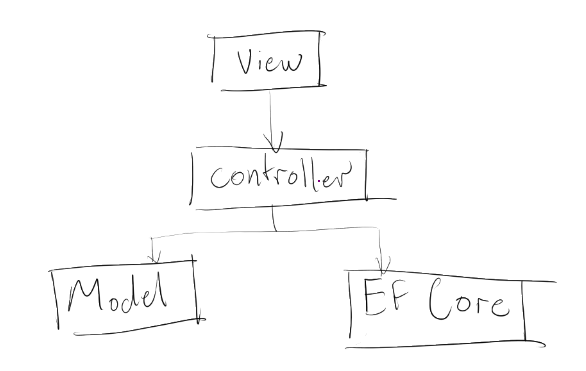
\includegraphics[width=1\textwidth]{billeder/simplecomponents.png}
	\caption{Simple component layer design}
\end{figure}

In the final design there will be several classes included within each of the components.
Each of the main classes in the model component will have a corresponding controller and view in relation to it.
For example the document class in the model component will have a corresponding database in EF Core and corresponding controller and view.
Here the documents object is within the model component and the documents data will be stored in the database.
A corresponding controller, which mainly handles the document class, ensures that the class and database are accessible for the actor.
A corresponding view ensures that the actor is able to see and interact with the document classes and database.
